\documentclass[letterpaper]{article}
\usepackage[submission]{aaai2027}
\usepackage[hyphens]{url}
\usepackage{graphicx}
\urlstyle{rm}
\def\UrlFont{\rm}
\usepackage{natbib}
\usepackage{caption}
\usepackage{booktabs}
\usepackage{amsmath}
\usepackage{amssymb}
\frenchspacing

\pdfinfo{
/TemplateVersion (2027.1)
}

\setcounter{secnumdepth}{0}

\title{MoSAIC: Modular Self-Attentive Interacting Columns for Recurrent Memory}
\author{Anonymous Submission}
\affiliations{}

\begin{document}

\maketitle

\begin{abstract}
Recurrent models preserve a fixed-size state, but conventionally organize it as one monolithic stream per layer. MoSAIC (Modular Self-Attentive Interacting Columns) instead factorizes state into persistent GRU columns and routes information among them with attention. Under approximately parameter-matched, one-billion-token training, this bias improves associative memory and character-level prediction. On Store--Distract--Query, L2C4 obtains $0.843 \pm 0.006$ long-gap final-window accuracy versus $0.532 \pm 0.103$ for a two-layer GRU, while L3C4 obtains $0.920 \pm 0.013$. On text8, L2C4 and L3C4 obtain $1.437 \pm 0.003$ and $1.435 \pm 0.002$ validation BPC, versus $1.483 \pm 0.006$ for the strongest GRU and $1.449 \pm 0.012$ for a similarly sized finite-context Transformer. These results support modular state organization as an inductive bias for recurrent computation at this scale.
\end{abstract}

\section{Introduction}

Recurrent networks compress sequence history into a fixed-size state and update it incrementally. A conventional GRU \citep{cho2014gru} or LSTM \citep{hochreiter1997lstm}, however, represents each layer as a single hidden-state stream. Width or depth adds capacity but leaves the organization and exchange of information within that state implicit.

We ask whether persistent modules with learned communication can organize a fixed recurrent budget. The goal is an explicit topology, not longer nominal context: components maintain local state while content-dependent routing moves information among them.

We introduce \emph{MoSAIC (Modular Self-Attentive Interacting Columns)}, which distributes each layer across independently parameterized GRU columns. Each column queries a small message bank before its recurrent update. The bottom layer reads the current input and delayed top-layer states; higher layers read the newly updated states below. All columns update, and the top layer persists to the next timestep.

This is modular state organization, not sparse expert selection. Column and layer counts organize recurrent state and computation, while attention over a fixed message set preserves fixed-size state as the sequence grows.

We evaluate at approximately ten million parameters on SDQ and text8 under a common one-billion-token horizon; text8 also includes matched finite-context Transformers. L2C4 is a compact reference and L3C4 the best observed shape, without designating a universal primary model.

Our contributions are:
\begin{itemize}
    \item \textbf{Architecture:} a layered grid of persistent recurrent columns with attention-mediated inter-column communication.
    \item \textbf{Controlled topology:} column count and depth provide explicit axes for organizing recurrent state and computation at roughly fixed parameter scale.
    \item \textbf{Empirical evidence:} matched GRU/MoSAIC comparisons show consistent improvements on SDQ and text8, and the text8 comparison includes a similarly sized finite-context Transformer.
\end{itemize}

\section{Related Work}

\paragraph{Modular recurrence and communication.}
Recurrent Independent Mechanisms (RIMs) \citep{goyal2019rims} maintain separate recurrent modules, sparsely activate a subset for each input, and allow active modules to communicate through attention. BRIMs \citep{mittal2020brims} add hierarchical bottom-up and top-down communication, while shared-workspace models \citep{goyal2021workspace} impose a communication bottleneck. Relational Memory Core \citep{santoro2018relational} instead updates interacting memory slots through attention. These works establish modular recurrence and learned communication as important design principles. MoSAIC differs in using a regular layered topology with dense synchronous updates: every persistent column updates at every timestep after reading from a layer-specific message bank. We therefore describe the mechanism as learned routing, not sparse or conditional computation.

\paragraph{Grid and multidimensional recurrence.}
Multi-Dimensional RNNs \citep{graves2007mdrnn} propagate information recurrently along multiple axes of structured data. Grid LSTM \citep{kalchbrenner2015gridlstm} arranges LSTM blocks in a multidimensional grid whose dimensions exchange hidden and memory vectors through fixed connections. MoSAIC uses a grid as an organization of modules rather than as an additional axis of the input. All columns share one temporal axis, retain separate recurrent states, and communicate through content-dependent routing rather than edges fixed by input geometry.

\paragraph{Modern recurrent and attention models.}
Recent architectures strengthen recurrent alternatives to full self-attention by redesigning the recurrent update or its memory representation. LRUs \citep{orvieto2023lru} stabilize long linear recurrences; HGRN2 \citep{qin2024hgrn2} expands the state of a gated linear RNN; Mamba-2 \citep{dao2024mamba2} connects selective state-space models with structured attention; DeltaNet \citep{yang2024deltanet} uses delta-rule matrix state; and xLSTM \citep{beck2024xlstm} includes scalar- and matrix-memory variants. Transformers \citep{vaswani2017attention} and segment-recurrent variants such as Transformer-XL \citep{dai2019transformerxl} instead retain a finite or growing bank of token representations for attention. MoSAIC keeps a conventional nonlinear GRU update and changes how recurrent state is divided and routed. Our experiments compare against GRUs and finite-context Transformers under the same token budget; memory-limited implementations of HGRN2, DeltaNet, and mLSTM are reported only under their separate reduced-token protocols.

\begin{figure*}[t]
\centering
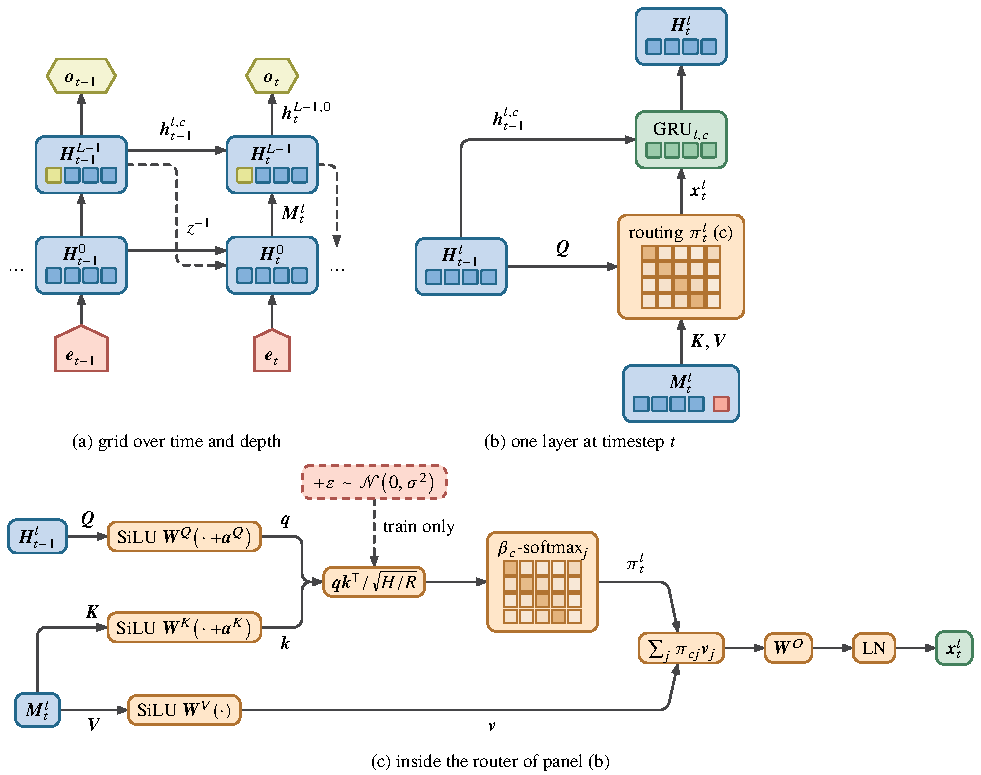
\includegraphics[width=0.94\textwidth]{fig_architecture.pdf}
\caption{MoSAIC mechanism. At timestep $t$, each persistent column state queries a layer-specific message bank. The first layer reads the current input together with the previous top-layer column states; later layers read the newly updated states below them. The routed message is the input to an independent recurrent update. All top-layer column states are carried to timestep $t+1$.}
\label{fig:architecture}
\end{figure*}

\section{Method}

\subsection{Persistent Columns and Layered Topology}

Let $\mathbf{e}_t \in \mathbb{R}^{B \times H}$ be an embedded input for a batch of size $B$. A conventional $L$-layer GRU maintains $\mathbf{S}_t \in \mathbb{R}^{L \times B \times H}$. MoSAIC instead maintains
\begin{equation}
    \mathbf{H}_t \in \mathbb{R}^{L \times C \times B \times H},
\end{equation}
where $\mathbf{h}_t^{l,c}$ denotes column $c$ at layer $l$. Each layer--column pair has independent GRU parameters. Columns in a layer are evaluated together for efficiency, but do not share recurrent weights.

The message bank for the first layer contains the delayed top layer and the current external inputs:
\begin{equation}
    \mathbf{M}_t^0 =
    [\mathbf{H}_{t-1}^{L-1}; \mathbf{e}_t^1; \ldots; \mathbf{e}_t^I]
    \in \mathbb{R}^{(C+I) \times B \times H}.
\end{equation}
Here $I$ is the number of input streams and $I=1$ in our experiments. At subsequent layers,
\begin{equation}
    \mathbf{M}_t^l = \mathbf{H}_t^{l-1}, \qquad l > 0.
\end{equation}
Information therefore moves bottom-up within a timestep, while the complete top layer provides a delayed feedback path across timesteps. Figure~\ref{fig:architecture} summarizes this computation.

\subsection{Attention-Mediated Routing}

At layer $l$, the previous states of its $C$ columns form the queries. Learnable identities distinguish query columns and message sources. For head $r$,
\begin{align}
\mathbf{q}_{t,c,r}^l &=
    \operatorname{SiLU}\!\left(
    \mathbf{W}_r^Q(\mathbf{h}_{t-1}^{l,c}+\mathbf{a}_c^Q)+\mathbf{b}_r^Q
    \right), \\
\mathbf{k}_{t,j,r}^l &=
    \operatorname{SiLU}\!\left(
    \mathbf{W}_r^K(\mathbf{m}_{t,j}^l+\mathbf{a}_j^K)+\mathbf{b}_r^K
    \right), \\
\mathbf{v}_{t,j,r}^l &=
    \operatorname{SiLU}\!\left(
    \mathbf{W}_r^V\mathbf{m}_{t,j}^l+\mathbf{b}_r^V
    \right).
\end{align}
Each query column has a learned positive inverse temperature $\beta_c=\operatorname{softplus}(\rho_c)$. The routing probabilities are
\begin{equation}
\pi_{t,c,j,r}^l =
\operatorname{softmax}_j\!\left[
\beta_c\left(
\frac{\mathbf{q}_{t,c,r}^l \cdot \mathbf{k}_{t,j,r}^l}{\sqrt{H/R}}
+ \epsilon_{t,c,j,r}^l
\right)\right],
\end{equation}
where $R$ is the number of heads. The perturbation $\epsilon$ is independent zero-mean Gaussian noise during training and zero at evaluation. Concatenated head outputs are linearly projected and layer-normalized:
\begin{equation}
\begin{aligned}
\mathbf{z}_{t,c,r}^l
    &= \sum_j \pi_{t,c,j,r}^l\mathbf{v}_{t,j,r}^l,
       &&r=1,\ldots,R,\\
\mathbf{x}_{t,c}^l
    &= \operatorname{LN}\!\left(
       \mathbf{W}^O[\mathbf{z}_{t,c,1}^l;\ldots;\mathbf{z}_{t,c,R}^l]
       \right).
\end{aligned}
\end{equation}
Routing determines the input to each recurrent cell; it does not replace or post-process its persistent state.

\subsection{Recurrent Update and Readout}

Every column performs an ordinary independent GRU update,
\begin{equation}
\mathbf{h}_t^{l,c} =
\operatorname{GRU}_{l,c}
(\mathbf{x}_{t,c}^l,\mathbf{h}_{t-1}^{l,c}).
\end{equation}
The prediction head reads column 0 of the top layer. All top-layer columns remain in the recurrent state and form part of the next bottom-layer message bank. This makes routing necessary for information stored outside the readout column to affect predictions.

The main configurations additionally use three training-only routing terms: Gaussian logit noise, a communication cost favoring diagonal routes, and an entropy bonus that discourages early route collapse. Let $S_l$ be the number of messages available at layer $l$. With zero-based column index $c$, the route cost $d_{c,j}^l$ is zero for the same-column recurrent message, one for another recurrent message, and $2c$ for the external input in the bottom layer. The communication loss is the mean expected route cost,
\begin{equation}
\mathcal{L}_{\mathrm{comm}}
= \mathbb{E}_{t,l,c,r}\!\left[
\sum_{j=1}^{S_l}\pi_{t,c,j,r}^l d_{c,j}^l
\right].
\end{equation}
Routing entropy is normalized by the log of the number of available messages,
\begin{equation}
\overline{\mathcal{H}}(\pi)
= \mathbb{E}_{t,l,c,r}\!\left[
\frac{-\sum_{j=1}^{S_l}\pi_{t,c,j,r}^l
\log \pi_{t,c,j,r}^l}{\log S_l}
\right].
\end{equation}
For task loss $\mathcal{L}_{\mathrm{task}}$,
\begin{equation}
\mathcal{L} =
\mathcal{L}_{\mathrm{task}}
+ \lambda_{\mathrm{comm}}\mathcal{L}_{\mathrm{comm}}
- \lambda_{\mathrm{ent}}\overline{\mathcal{H}}(\pi).
\end{equation}
All MoSAIC configurations use four routing heads. For text8, $(\lambda_{\mathrm{comm}},\lambda_{\mathrm{ent}},\sigma_\epsilon)=(0.05,0.005,0.05)$; for SDQ, the settings are $(0.02,0.002,0.02)$. These terms add no inference-time state and are not treated as separate empirical contributions in the absence of completed component ablations.

\subsection{Fixed-State and Resource Accounting}

Attention is applied over $C+I$ messages in the bottom layer and $C$ messages above it, rather than over token history. For fixed $L$, $C$, and $H$, MoSAIC therefore carries a fixed-size recurrent state and supports incremental processing as sequence length grows. This is an architectural property, not an empirical claim of superior long-context scaling.

Ignoring embeddings and biases, the independent GRUs contribute approximately $6LCH^2$ parameters and routing projections approximately $4LH^2$. Persistent state contains $LCH$ scalars per example, compared with $LH$ for a stacked GRU. Parameter matching consequently does not match activation state or computation. We report recurrent-state size to make this distinction explicit, but do not claim resource efficiency.

\begin{table*}[t]
\centering
\begin{tabular}{llrcrr}
\toprule
Family & Shape & Params & $n$ & Endpoint & Final-five \texttt{Acc++} $\uparrow$ \\
\midrule
GRU & L1 & 10.18M & 3 & 970M & $0.6177 \pm 0.0052$ \\
GRU & L2 & 10.06M & 2 & 980M & $0.5322 \pm 0.1027$ \\
GRU & L3 & 10.25M & 2 & 990M & $0.2865 \pm 0.0798$ \\
\midrule
MoSAIC & L1C8 & 10.12M & 3 & 1000M & $0.7051 \pm 0.0163$ \\
MoSAIC & L2C4 & 10.12M & 3 & 985M & $0.8433 \pm 0.0055$ \\
MoSAIC & L2C8 & 10.18M & 3 & 1000M & $0.8664 \pm 0.0099$ \\
MoSAIC & L2C16 & 10.09M & 1 & 1000M & $0.8901$ \\
MoSAIC & L3C4 & 9.99M & 3 & 1000M & $\mathbf{0.9204 \pm 0.0128}$ \\
\bottomrule
\end{tabular}
\caption{Matched SDQ results under the one-billion-token target. ``Endpoint'' is the final logged point used for each configuration under the logging-loss convention. Values are mean $\pm$ standard deviation of replicate-level final-five \texttt{Acc++} averages.}
\label{tab:sdq}
\end{table*}

\section{Experiments}

\subsection{Shared Protocol and Reporting}

All principal GRU and MoSAIC configurations are approximately parameter matched at ten million trainable parameters. The principal horizon is one billion processed tokens. Runs with a final logged evaluation point slightly below one billion are retained only under the documented logging-loss convention; longer runs are truncated at the one-billion-token horizon. Results report the mean and standard deviation across completed replicates. We make no statistical-significance claim.

L2C4 is the compact reference configuration used for direct two-layer comparisons. L3C4 is the best observed configuration in both tasks. The shape sweep is reported in full rather than using rhetoric to designate either as a universal primary model.

\subsection{Store--Distract--Query}

\paragraph{Task.}
SDQ is an online synthetic task designed to isolate associative storage and retrieval under interference. With five keys and ten values, the vocabulary comprises 50 key--value store tokens, ten distractor tokens, and five query tokens. A store overwrites the value associated with its key. Distractor values contribute to a running sum modulo ten. At a query, the target combines the current stored value, the distractor sum, and the configured per-key store and query counts. Cross-entropy is applied only at query events.

Episode lengths are geometrically distributed. During training, their mean increases from 10 toward 500, while store and query probabilities decrease from 0.35 toward 0.10 and 0.25. Models use 512 parallel streams, a truncation length of 32, RMSprop, gradient clipping at norm 1, and the same learning-rate schedule and online generator.

\paragraph{Metric.}
The code logs \texttt{Acc++} as query accuracy on examples whose valid store--query gaps are above the current batch mean. This emphasizes the longer-gap half of non-missing queries. For each completed replicate, we average the final five logged \texttt{Acc++} values through the one-billion-token horizon and then aggregate those replicate-level averages.

\paragraph{Results.}
Table~\ref{tab:sdq} shows a consistent family-level advantage for MoSAIC: every evaluated shape has a higher central \texttt{Acc++} value than every GRU depth. In the replicated two-layer comparison, L2C4 reaches $0.8433 \pm 0.0055$, while GRU-L2 reaches $0.5322 \pm 0.1027$. L3C4 is the best observed configuration at $0.9204 \pm 0.0128$. L2C16 remains a single-replicate observation and therefore provides limited evidence about run-to-run variability.

\begin{figure*}[t]
\centering
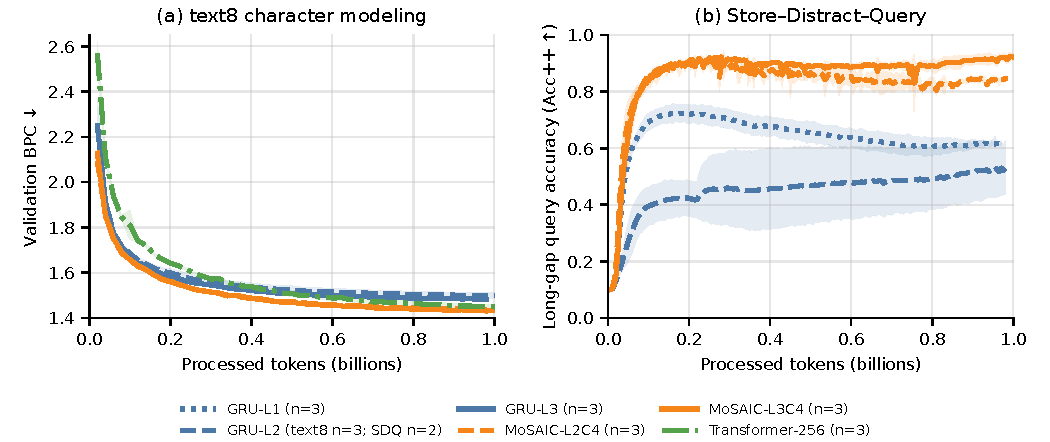
\includegraphics[width=0.96\textwidth]{fig_learning_curves.pdf}
\caption{Learning dynamics under the standard 1B-token protocol. Lines show the mean across completed replicates and shading shows $\pm 1$ standard deviation. Text8 curves use three replicates; SDQ curves use three except GRU-L2, which uses two. (a) Validation BPC on text8. (b) Online long-gap query accuracy on SDQ. Final SDQ values in Table~\ref{tab:sdq} use the mean of each replicate's last five logged values.}
\label{fig:learning-curves}
\end{figure*}

\begin{table*}[t]
\centering
\begin{tabular}{llrcrr}
\toprule
Family & Shape / cache & Params & $n$ & Endpoint & Validation BPC $\downarrow$ \\
\midrule
GRU & L1 & 10.16M & 3 & 980M & $1.5626 \pm 0.0028$ \\
GRU & L2 & 10.04M & 3 & 1000M & $1.5004 \pm 0.0119$ \\
GRU & L3 & 10.23M & 3 & 980M & $1.4828 \pm 0.0062$ \\
\midrule
MoSAIC & L1C8 & 10.11M & 3 & 1000M & $1.4687 \pm 0.0046$ \\
MoSAIC & L2C4 & 10.11M & 3 & 980M & $1.4367 \pm 0.0026$ \\
MoSAIC & L2C8 & 10.17M & 3 & 1000M & $1.4452 \pm 0.0019$ \\
MoSAIC & L2C16 & 10.09M & 2 & 1000M & $1.4548 \pm 0.0023$ \\
MoSAIC & L3C4 & 9.99M & 3 & 1000M & $\mathbf{1.4345 \pm 0.0017}$ \\
\midrule
Transformer & cache 256 & 10.07M & 3 & 1000M & $1.4492 \pm 0.0120$ \\
Transformer & cache 64 & 10.07M & 3 & 962.6M & $1.4826 \pm 0.0057$ \\
\bottomrule
\end{tabular}
\caption{Fixed-horizon text8 results under the one-billion-token target. ``Endpoint'' is the final logged validation point used for each configuration. The Transformer cache variants are distinct configurations, not replicates.}
\label{tab:text8}
\end{table*}

\subsection{Character-Level Modeling}

\paragraph{Data and training.}
Text8 \citep{mahoney2011text8} contains 100 million normalized English characters with a 27-character alphabet. We use the first 90 million characters for training and the final 10 million as a contiguous validation split. The validation split was used for limited manual configuration tuning, so we call the metric validation BPC rather than an untouched test estimate.

GRU and MoSAIC models process 512 parallel contiguous streams with truncated backpropagation through time over 64 steps. Random state resets decay from probability $0.2/64$ toward $0.001/64$ per token, increasing the expected uninterrupted context from about 320 to 64,000 characters. Models use RMSprop, a learning rate warming to $5 \times 10^{-4}$ and decaying toward $5 \times 10^{-5}$, and gradient clipping at norm 1. Validation runs disable random resets and evaluate contiguous streams.

The Transformer uses the same tokenization, data split, reset schedule, optimizer, token batch per update, and one-billion-token budget. It has four layers, hidden width 560, four attention heads, feed-forward width 1120, RMSNorm, and rotary position embeddings (RoPE). It processes each 64-token training segment in parallel and carries a rolling valid key/value cache of 256 or 64 tokens between segments; the two cache lengths are distinct configurations.

\paragraph{Results.}
As shown in Table~\ref{tab:text8}, every evaluated MoSAIC shape has a lower central BPC than every matched GRU. The compact L2C4 reference reaches $1.4367 \pm 0.0026$, compared with $1.5004 \pm 0.0119$ for GRU-L2. L3C4 is the best observed shape at $1.4345 \pm 0.0017$; the strongest GRU, L3, reaches $1.4828 \pm 0.0062$. The cache-256 Transformer reaches $1.4492 \pm 0.0120$ under the same token budget. Thus the observed MoSAIC means are lower while retaining recurrent fixed-state operation; this comparison does not establish general Transformer superiority or long-context scaling.

\subsection{Topology and State Allocation}

Parameter matching changes hidden width and persistent-state size. Table~\ref{tab:topology} isolates those differences for the recurrent families. At two layers, increasing MoSAIC from four to eight and sixteen columns increases state size while worsening text8 BPC relative to L2C4. L2C16 stores more than twice as many recurrent scalars as L2C4 but obtains a higher BPC. On SDQ, the central values increase across these shapes, although L2C16 has only one completed run. Depth also behaves differently across families: L3C4 improves over L2C4 on both tasks, whereas deeper GRUs improve on text8 but not SDQ. These observations show that state volume alone does not explain the results and that the allocation across depth, column count, and within-column width matters.

\begin{table}[t]
\centering
\small
\begin{tabular}{lrrr}
\toprule
Shape & $H$ & State & Params \\
\midrule
GRU-L1 & 1,296 & 1,296 & 10.16M \\
GRU-L2 & 912 & 1,824 & 10.04M \\
GRU-L3 & 752 & 2,256 & 10.23M \\
\midrule
L1C8 & 440 & 3,520 & 10.11M \\
L2C4 & 424 & 3,392 & 10.11M \\
L2C8 & 312 & 4,992 & 10.17M \\
L2C16 & 224 & 7,168 & 10.09M \\
L3C4 & 344 & 4,128 & 9.99M \\
\bottomrule
\end{tabular}
\caption{Recurrent topology and persistent-state scalars per example for text8 configurations. SDQ uses the same hidden widths and shapes, with small parameter-count differences from its input and output vocabularies.}
\label{tab:topology}
\end{table}

\paragraph{Reduced-token baselines.}
HGRN2, DeltaNet, and mLSTM exceeded available memory at the standard 512-stream geometry. Their completed runs therefore use different token, batch, and update budgets from the one-billion-token comparisons. We retain them only as non-comparable implementation context and draw no relative quality or efficiency conclusion from them.

\section{Discussion and Limitations}

Across the controlled comparisons, MoSAIC's columnar topology is associated with better associative-memory and character-modeling results than monolithic recurrent baselines at approximately fixed parameter scale. The pattern is consistent across the evaluated shapes rather than depending only on the best run family member. The text8 result relative to the finite-context Transformer provides additional context: MoSAIC retains recurrent fixed-state operation and obtains a lower mean BPC under the present matched token budget.

These results support a narrow conclusion. They do not show that columns acquire identifiable functional roles, that dense routing behaves as sparse expert selection, or that MoSAIC replaces Transformers generally. The architecture permits incremental inference with state size independent of processed sequence length, but the experiments do not establish superior long-context scaling or long-horizon retention against all alternatives.

Parameter matching also leaves important resources unmatched. MoSAIC exposes more persistent state coordinates than the GRUs and performs routing computation at every layer and timestep. We have not completed controlled throughput, peak-memory, or inference-latency measurements, so the results should be interpreted as evidence about an architectural inductive bias rather than resource efficiency. Likewise, the reduced-token recurrent baselines use different token and update budgets and are not direct quality comparisons.

The empirical scope is limited. Text8 is a small character-level corpus, its validation split received limited manual tuning, and the study operates at roughly ten million parameters. SDQ is synthetic and uses a curriculum-controlled online generator. SDQ L2C16 has one completed run, text8 L2C16 has two, and the current SDQ GRU-L2/L3 aggregates use two runs; we make no statistical-significance claims. Training-only routing regularizers add hyperparameters whose individual effects have not been isolated. Finally, the present paper omits reinforcement-learning results because the task-matched evidence is incomplete and variable.

\section{Conclusion}

MoSAIC factorizes a monolithic recurrent state into persistent columns and learns how information is routed among them before independent recurrent updates. Under controlled, approximately parameter-matched one-billion-token training, this structural bias consistently improves associative memory and character-level modeling over monolithic GRUs. A similarly sized finite-context Transformer provides a matched text8 reference, while the separate reduced-token results are reported only as non-comparable implementation context. The evidence supports modular state organization as a useful inductive bias for recurrent computation at this scale; broader claims about specialization, long-context scaling, and resource efficiency remain open.

\bibliography{refs}

\end{document}
